\section{Description of the software structure and functionality}

The following section will introduce the software segment, based on our required specifications. The design will shown in the form of a flowchart.
TBD Softwarebeskrivelse og underafsnit

\section {Description of the PID controller} 
 
A PID controller continuously calculates an error value as the difference to a reference point and a measured process variable.\\
PID is an abbreviation for a proportional-integral-derivative controller, it is a control loop feedback mechanism. The controllers job is to minimize the error value for the given devices running time. In the case of this project the reference point is the line to follow and the PID will allow the MCU to adjust the power to the engines, to steer accordingly to said reference point.
$$\mathrm{F}(t)=K_p{e(t)} + K_{i}\int_{0}^{t}{e(\tau)}\,{d\tau} + K_{d}\frac{de(t)}{dt}$$

\begin{figure}[h!]
  \centering
  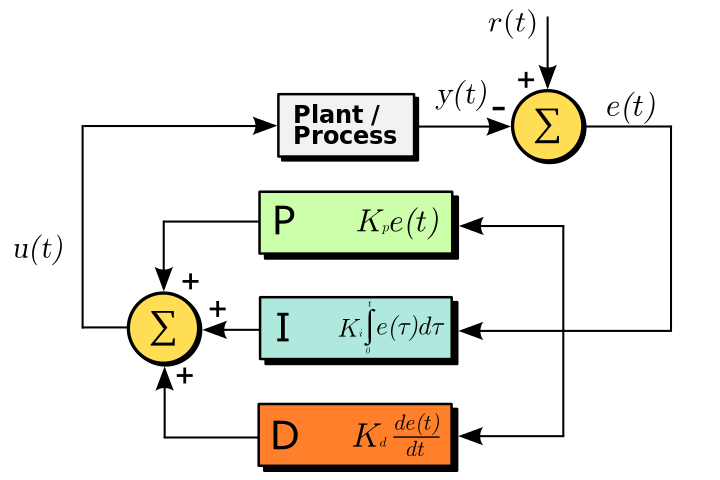
\includegraphics[width=0.5\textwidth]{figures/PID_block.png}
  
  \caption{Block diagram, showing the idea of PID controller. Credits: %https://en.wikipedia.org/wiki/PID_controller#/media/File:PID_en_updated_feedback.svg
  }
  \label{PID controller}
\end{figure}

\subsection {Proportional control(P)}

The proportional part creates an output value that is proportionally related to the current error value, this value can be tuned by multiplying the error by a constant $K_p$. A high proportional gain results in a large change in the output for a given change in the error. 


$$ P_{\mathrm{out}}=K_p\,{e(t)}$$  

If the proportional gain is too high, the system can become unstable. Contrarily, a small gain will result in the device adjusting too slowly, which decreases overall efficiency and in the case of this project, it will end up being detrimental to the steering accuracy.


\begin{figure}[h!]
  \centering
  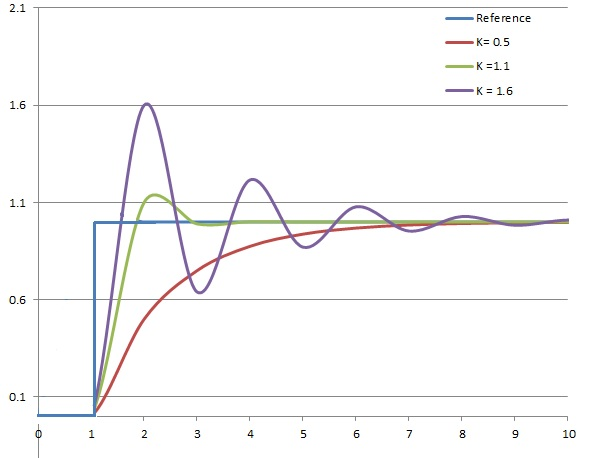
\includegraphics[width=0.5\textwidth]{figures/PIDP.jpg}
  
  \caption{$K_p$ with 3 values. ($K_i$, $K_d$ held constant) Credits: %https://en.wikipedia.org/wiki/PID_controller#/media/File:PID_varyingP.jpg
  }
  \label{PID controller}
\end{figure}

\subsection {Steady-state error}
TBD (omskrives)
%Because a non-zero error is required to drive it, a proportional controller generally operates with a so-called steady-state error.[a] Steady-state error (SSE) is proportional to the process gain and inversely proportional to proportional gain. SSE may be mitigated by adding a compensating bias term to the setpoint or output, or corrected dynamically by adding an integral term.

\subsection {Integral control(I)}

The integral controller is contributing proportionally to both the magnitude of the error and the duration of the error. \\
The integral in a PID controller is the sum of the instantaneous error over time and gives the accumulated offset that should have been corrected previously. \\ 

The controller output equals the accumulated error multiplied by the integral gain(Ki)\\
$$I_{\mathrm{out}}=K_{i}\int_{0}^{t}{e(\tau)}\,{d\tau}$$ 

The integral part accelerates the movement of the process towards the reference point.
Since the integral term correlates to accumulated errors from the past, it can cause the present value to overshoot the reference value.

\subsection {Derivative control(D)} 

The derivative of the process error is calculated by determining the slope of the error over time and multiplying this rate of change by the derivative gain $K_d$. The magnitude of the contribution of the derivative term to the overall control action is termed the derivative gain, $K_d$.
\begin{figure}[h!]
  \centering
  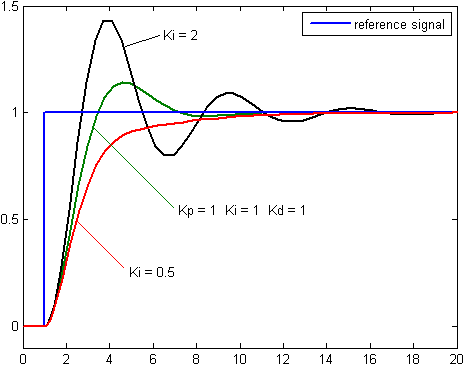
\includegraphics[width=0.5\textwidth]{figures/Change_with_Ki.png}
  
  \caption{$K_i$ shown with 3 values. Credits: %https://en.wikipedia.org/wiki/PID_controller#/media/File:Change_with_Ki.png
  }
  \label{PID controller}
\end{figure}

TBD (billede skal rettes ind til teksten)
The derivative term is given by:

$$D_{\mathrm{out}}=K_d\frac{de(t)}{dt}$$
The derivative action predicts system behaviour and utilizes this to improve the settling time and stability of the system.
An ideal derivative is not causal, so that implementations of PID controllers include an additional low pass filtering for the derivative term, to limit the high frequency gain and noise.

\begin{figure}[h!]
  \centering
  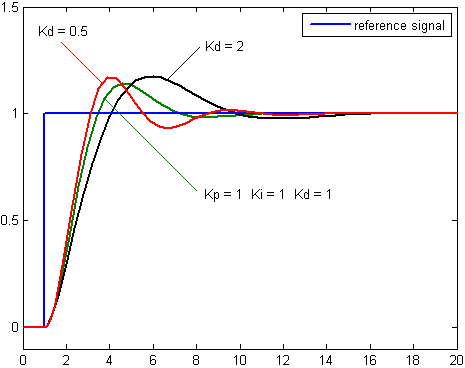
\includegraphics[width=0.5\textwidth]{figures/Change_with_Kd.png}
  
  \caption{$K_d$ shown with 3 values. Credits: %https://en.wikipedia.org/wiki/PID_controller#/media/File:Change_with_Kd.png
  }
  \label{PID controller}
\end{figure}



\subsection {Loop tuning} 

Tuning the loop is the term used to describe the adjustments of the PID’s control parameters (proportional band/gain, integral gain/reset, derivative gain/rate) to the optimal values for the given control scheme. \\ Stability is the first requirement; however systems can differ greatly, and different applications may have different requirements and these may even conflict with each other. For example, high speed and high accuracy often cancel each other out, because high speed may cause overshooting, while high accuracy is slow.\\ The ideal realistic behaviour is both as fast as possible, while also having minimum overshoot and oscillation. \\ 

Even though the process seems simple, with only three variables, it can be challenging to achieve, because it must satisfy the criteria despite being within the limitations of PID control. While adjusting the PID can seem conceptually intuitive, and while most PIDs may perform acceptably with default controls, they may very well also have an unsatisfactory performance.\\ This can generally be fixed through optimisation and tuning, either through computer simulations or manual testing. In our case, we used manual tuning of the numbers.

\subsection {Stability} 

If the parameters of the PID controller are set incorrectly the process input can become unstable.
This means the controllers output becomes divergent, which can be limited by saturation and mechanical breaking. \\

\subsection {Manual tuning} 

When a system must be online at all times a method for tuning is to first set $K_i$ and $K_d$ values to zero. Increase $K_p$ until the loop output oscillates, setting $K_p$ at approximately half the value for a "quarter amplitude decay" type response.\\ 
Then increase $K_i$ until any set off is corrected in sufficient time for the process. Adding too much $K_i$ will however cause an instability. 
Finally, increase $K_d$, if required at all, until the loop is acceptably quick to reach its reference after a load disturbance.
\\ 
A fast PID loop tuning process usually overshoots slightly to reach the reference point faster.\\ %Kan vi få en kilde på det?
In the case of systems that can't accept overshoot, an over-damped closed-loop system is best suited, which requires $K_p$ setting significantly less than half that of the $K_p$ setting that was causing the oscillation.
\\TBD kilde (http://blog.opticontrols.com/archives/1066)

TBD (Vores fremgangsmåde med PID alt efter om "D" skal bruges)

\begin{table}[h]
\centering
\caption{Manual tuning}
\label{Table: Manual tuning}
\begin{tabular}{|l|l|l|l|l|l|}
\hline
\rowcolor[HTML]{C0C0C0} 
{\color[HTML]{000000} Parameter}                     & Rise time    & Overshoot & Settling time & Steady-state error  & Stability              \\ \hline
\cellcolor[HTML]{C0C0C0}{\color[HTML]{000000} $K_p$} & Decrease     & Increase  & Small change  & Decrease            & Degrade                \\ \hline
\cellcolor[HTML]{C0C0C0}{\color[HTML]{000000} $K_i$} & Decrease     & Increase  & Increase      & Eliminate           & Degrade                \\ \hline
\cellcolor[HTML]{C0C0C0}{\color[HTML]{000000} $K_d$} & Minor change & Decrease  & Decrease      & \begin{tabular}[c]{@{}l@{}}No effect\\ in theory\end{tabular} & \begin{tabular}[c]{@{}l@{}}Improves if\\ $K_d$ is small\end{tabular} \\ \hline
\end{tabular}
\end{table}

\subsubsection {Table 3.1 explained}

Table 3.1 gives an informative overview of what the different parameters does when tuned manually.

\begin{enumerate}
		\item[•]To minimize the rise time, decrease $K_p$
		\item[•]To eliminate the steady-state error, increase $K_i$
		\item[•]To reduce the overshoot and settling time, decrease $K_d$
	\end{enumerate}

\section{Description of the Pulse Width Modulator - PWM}

A pulse width modulation technique used to encode a message into a pulsing signal. Its primary use is to control the power supply of electronic devices - the case of this project; this means the motors.\
The average voltage and amplitude output to the motors is altered by rapidly switching between an 'on' and 'off' state. This way, the average output is easily altered by changing the proportions between the on and off state. The longer the switch is set to on compared to off, the higher the average supply will be.\\

$$\overline{y}=\frac{1}{T}\int_{0}^{T}f(t)dt$$\\
 
 $$\overline{y}=\frac{1}{T}\left(\int_{0}^{DT}y_\mathrm{max}dt+\int_{DT}^{T}y_\mathrm{min}dt\right)$$
 $$=\frac{1}{T}\left(D \cdot T \cdot y_\mathrm{max}+T(1-D)y_\mathrm{min}\right)$$
 $$=D \cdot y_\mathrm{max}+\left(1-D\right)y_\mathrm{min}$$\\
 
 TBD forklaring af ligninger

\subsection{Duty cycles}
 The duty cycle describes the proportion of 'on' compared to any given period of runtime for the device. The duty cycle is described as a percentage, where 100\% means that it's turned on the entire time, where 10\% would be a tenth of the time.\\
 TBD Vores duty cycle\\
 
 